\documentclass[12pt,a4paper]{article}

% Course template packages and layout
\usepackage{amsmath,amsthm,amssymb}
\usepackage{graphicx}
\usepackage{booktabs}
\usepackage{geometry}
\usepackage{natbib}
\usepackage{hyperref}
\usepackage{color}
\usepackage{enumitem}
\usepackage{multirow}
\usepackage{url}
\usepackage{array}
\usepackage{float}
\newcommand{\FloatBarrier}{\par}
\geometry{left=2.2cm,right=2.2cm,top=2.2cm,bottom=2.2cm}
\hypersetup{
    colorlinks=true,
    hypertexnames=false,
    linkcolor=blue,
    filecolor=magenta,
    urlcolor=cyan,
    citecolor=blue
}

\newtheorem{theorem}{Theorem}[section]
\newtheorem{lemma}[theorem]{Lemma}
\newtheorem{proposition}[theorem]{Proposition}
\newtheorem{corollary}[theorem]{Corollary}
\newtheorem{definition}[theorem]{Definition}
\newtheorem{remark}[theorem]{Remark}

\title{\vspace{-1.1cm}\textbf{\huge Controlling Smoothness in Nonparametric Regression: \\Theory, Simulations, and \\Real Data Analysis}}
\author{Ding Yuxia \quad PB23611962}
\date{\today}

\begin{document}
\renewcommand{\baselinestretch}{1.18}\normalsize
\setlength{\parindent}{0pt}
\setlength{\parskip}{0.28em}
\maketitle

\begin{abstract}
Nonparametric smoothing methods estimate unknown densities or regression functions without imposing a finite-dimensional parametric specification. Their flexibility is statistically useful only when it is accompanied by explicit complexity control. This paper reviews kernel density estimation, Nadaraya-Watson regression, local polynomial regression, B-spline regression, and smoothing splines from a common perspective: smoothing parameters regulate the bias-variance trade-off. In kernel density estimation and kernel regression this parameter is the bandwidth; in local polynomial regression it determines the local neighborhood; in spline methods it appears as the number of knots, the basis dimension, or a roughness penalty. The main formulas are stated in the text, while longer derivations are placed in the appendix. Numerical experiments examine bandwidth sensitivity, method-specific behavior under different regression functions, and the effect of heavy-tailed, heteroscedastic, and contaminated noise. An exploratory analysis of the Bike Sharing Dataset illustrates nonlinear temperature effects and also shows the limitations induced by temporal structure and count responses. The results do not identify a uniformly dominant smoother; rather, they show that the choice of smoother and smoothing parameter should be linked to the inferential goal, the design distribution, and the noise structure.
\end{abstract}

\noindent\textbf{Keywords:} nonparametric regression; smoothing methods; bias-variance trade-off; Bike Sharing dataset.

\setcounter{tocdepth}{2}
\tableofcontents

\section{Introduction}

Statistical modeling often begins with an unknown density \(f(x)\) or an unknown regression function \(m(x)=E(Y\mid X=x)\). In transportation, environmental, economic, and engineering data, such functions are rarely exactly linear. They may contain curvature, local peaks, boundary effects, or changing variance. This paper focuses on one-dimensional exploratory nonparametric smoothing, where the objective is to estimate the shape of an unknown curve without treating a simple parametric form as correct.

Parametric models remain valuable because they are stable and interpretable. A linear model, for example, gives a concise summary of a relationship, and a low-order polynomial can introduce limited curvature. The price is model specification. If the actual curve has local structure that the chosen parametric family cannot represent, the fitted curve has systematic bias. Increasing the polynomial degree may reduce this bias, but it can also create unstable boundary behavior and weaker interpretability.

Nonparametric smoothing weakens functional-form assumptions, but it does not remove the need for structure. A highly flexible smoother may track random noise and exhibit high variance. An excessively smooth estimator may remove genuine local features and exhibit high bias. The central statistical question is therefore not only how to construct a flexible estimator, but also how to choose the extent of smoothing.

The methods considered here are chosen to make this question visible; standard references include \citet{hardle1990applied}, \citet{wasserman2006all}, and \citet{tsybakov2009introduction}. Kernel density estimation (KDE) gives the cleanest theoretical example of bandwidth, bias, variance, AMISE, and optimal rate \citep{rosenblatt1956remarks,parzen1962estimation,silverman1986density,wand1995kernel}. The Nadaraya-Watson estimator transfers kernel smoothing to regression through a local weighted average \citep{nadaraya1964estimating,watson1964smooth}. Local polynomial regression improves local constant smoothing by fitting a Taylor approximation in each neighborhood \citep{fan1996local}. B-spline regression and smoothing splines use basis functions and roughness penalties to estimate a whole curve at once \citep{deboor2001practical,eilers1996flexible,craven1979smoothing,wahba1990spline,green1994nonparametric}.

The paper is intended as a review plus empirical comparison. First, it organizes these methods under the common principle that smoothing parameters control the bias-variance trade-off. Second, it states the main mathematical forms in the text and places longer derivations in Appendix~A. Third, it uses simulations to study bandwidth sensitivity, differences among smoothers, and sensitivity to noise structure. Finally, it analyzes the Bike Sharing Dataset \citep{fanaee2014event} as an exploratory real-data example.

The rest of the paper is organized as follows. Section~\ref{sec:principle} states the general smoothing principle. Section~\ref{sec:kde} discusses KDE and bandwidth. Section~\ref{sec:regression} introduces nonparametric regression methods, with the methodological comparison given in Subsection~\ref{sec:comparison}. Sections~\ref{sec:simulation} and~\ref{sec:realdata} present simulations and the Bike Sharing analysis. Section~\ref{sec:discussion} discusses limitations and extensions, and Section~\ref{sec:conclusion} concludes. Appendix~A gives theoretical derivations, Appendix~B gives supplementary simulations, and Appendix~C describes the code implementation.

\section{General Principle of Nonparametric Smoothing}
\label{sec:principle}

Suppose observations \((X_i,Y_i)\), \(i=1,\ldots,n\), are available and the target is a regression function \(m(x)=E(Y\mid X=x)\). The density estimation problem is similar, with target \(f(x)\). Nonparametric smoothing does not specify \(m\) or \(f\) by a finite-dimensional parameter. Instead, it estimates the curve directly while imposing smoothness to avoid completely unrestricted interpolation.

The local mean squared error at a fixed point has the standard decomposition
\[
E\{(\hat m_s(x)-m(x))^2\}
=\operatorname{Bias}^2\{\hat m_s(x)\}
+\operatorname{Var}\{\hat m_s(x)\},
\]
where \(s\) denotes a smoothing parameter. In typical smooth-function settings, weaker smoothing reduces approximation bias but increases sampling variability, whereas stronger smoothing stabilizes the estimator at the cost of potentially larger bias. The same principle appears throughout the paper, although the parameter \(s\) has different forms.

In KDE and kernel regression, \(s\) is the bandwidth \(h\). It determines the size of the local window. In local polynomial regression, \(h\) again determines the neighborhood, while the polynomial degree \(p\) determines the local approximation. In B-spline regression, the number and placement of knots determine the basis dimension. In smoothing splines, the roughness penalty \(\lambda\) controls the degree of smoothing, and the effective degrees of freedom give an interpretable measure of complexity.

A second distinction is between local and global smoothers. Local methods such as Nadaraya-Watson and local polynomial regression refit the curve around each target point. Global methods such as B-spline regression and smoothing splines define the entire fitted curve through a basis expansion or an optimization problem. Both approaches control complexity, but they do so with different computational and statistical consequences.

Many estimators considered below can also be viewed as linear smoothers. For a fixed value of the smoothing parameter, the fitted values at the design points can often be written as
\[
\hat{\mathbf y}=S_s\mathbf y,
\]
where \(S_s\) is a smoothing matrix depending on the design points and on the smoothing parameter \(s\). This representation is useful because it separates the statistical role of the response vector from the structural role of the smoother. A rough measure of model complexity is \(\operatorname{tr}(S_s)\), the effective degrees of freedom. For kernel methods this trace typically increases as the bandwidth decreases; for smoothing splines it decreases as the penalty parameter \(\lambda\) increases. Thus bandwidth, basis dimension, and penalty strength can all be interpreted as different parameterizations of complexity control.

This perspective also clarifies why the goal of smoothing is not interpolation. In an unrestricted interpolation problem, the fitted values may match the observations exactly, but the resulting curve can be dominated by noise. A smoother deliberately sacrifices exact fit in order to reduce variance and produce a curve that is more stable under repeated sampling. The central issue is therefore not whether the fitted curve passes through the data, but whether the chosen amount of smoothing is appropriate for the scale of the signal one wishes to recover. Before moving to regression, it is useful to examine KDE, where the bias and variance orders can be derived cleanly.

\section{Kernel Density Estimation and Bandwidth}
\label{sec:kde}

\subsection{Definition}

Let \(X_1,\ldots,X_n\overset{i.i.d.}{\sim}F\) and assume \(F\) has density \(f\). A kernel density estimator is
\[
\hat f_h(x)=\frac{1}{n}\sum_{i=1}^{n}K_h(x-X_i),
\qquad
K_h(u)=\frac{1}{h}K\left(\frac{u}{h}\right).
\]
Here \(K\) is a kernel and \(h>0\) is the bandwidth. Typical assumptions are that \(K\) is nonnegative, symmetric, integrates to one, and has finite second moment.

The bandwidth is the key smoothing parameter. If \(h\) is small, the estimate reacts strongly to individual observations. If \(h\) is large, the estimate averages over a wide region and suppresses local detail. This is the simplest setting in which the bias-variance trade-off becomes explicit.

\subsection{Bias, Variance, and AMISE}

Under the usual smoothness and kernel moment conditions,
\[
\operatorname{Bias}\{\hat f_h(x)\}=O(h^2),
\qquad
\operatorname{Var}\{\hat f_h(x)\}=O((nh)^{-1}).
\]
The proof is given in Appendix~A1. The result says that increasing \(h\) raises the leading bias order but lowers the leading variance order. This is the mathematical form of the qualitative smoothing trade-off.

The integrated squared error and mean integrated squared error are
\[
\operatorname{ISE}(h)=\int\{\hat f_h(x)-f(x)\}^2dx,
\qquad
\operatorname{MISE}(h)=E[\operatorname{ISE}(h)].
\]
Keeping only leading terms gives the AMISE approximation
\[
\operatorname{AMISE}(h)\approx C_1h^4+\frac{C_2}{nh},
\]
where \(C_1\) depends on the curvature of \(f\) and \(C_2\) depends on the kernel. Minimizing this expression gives
\[
h_{\mathrm{opt}}\asymp n^{-1/5}.
\]
The rate is slow: even with larger samples, the optimal bandwidth should decrease cautiously.

Common practical choices include rule-of-thumb bandwidths, plug-in methods, and cross-validation \citep{silverman1986density,scott2015multivariate,wand1995kernel}. The kernel choice also matters, but among reasonable kernels its effect is usually secondary to the bandwidth. The simulations therefore fix a standard kernel and focus on smoothing parameters and method structure.

The asymptotic result should not be read as a complete bandwidth-selection rule. The rate \(n^{-1/5}\) describes how the optimal order changes with sample size, but the multiplicative constant depends on unknown features such as \(R(f'')\). In practice, a rule-of-thumb bandwidth substitutes a simple reference distribution; a plug-in method estimates the unknown curvature terms; and cross-validation selects the bandwidth by empirical predictive performance. These approaches can produce different values in finite samples. This is one reason the simulation study reports both fitted curves and risk summaries rather than treating one selected bandwidth as automatically definitive.

Table~\ref{tab:kde-facts} summarizes the key asymptotic facts used later to interpret bandwidth selection and the simulation results.

\begin{table}[htbp]
\centering
\caption{Main KDE facts used in the paper.}
\label{tab:kde-facts}
\begin{tabular}{lll}
\toprule
Quantity & Main order or form & Role \\
\midrule
Bias & \(O(h^2)\) & increases with bandwidth \\
Variance & \(O((nh)^{-1})\) & decreases with bandwidth \\
AMISE & \(C_1h^4+C_2/(nh)\) & integrated approximation \\
Optimal bandwidth & \(h_{\mathrm{opt}}\asymp n^{-1/5}\) & balances leading terms \\
\bottomrule
\end{tabular}
\end{table}

\section{Nonparametric Regression Methods}
\label{sec:regression}

The density-estimation discussion shows how bandwidth controls smoothing. Regression estimators use the same principle but target \(m(x)=E(Y\mid X=x)\). This section introduces the methods compared later in the simulations and real data analysis.

\subsection{Nadaraya-Watson Estimator}

Given observations \((X_i,Y_i)\), the Nadaraya-Watson estimator is
\[
\hat m_h(x)=
\frac{\sum_{i=1}^n K_h(X_i-x)Y_i}
{\sum_{i=1}^n K_h(X_i-x)}
=\sum_{i=1}^n W_i(x)Y_i,
\]
where
\[
W_i(x)=
\frac{K_h(X_i-x)}
{\sum_{j=1}^n K_h(X_j-x)}.
\]
The weights are nonnegative and sum to one. Thus the estimate is a local weighted average of the responses. Points near \(x\) receive larger weights.

This estimator can be derived by writing \(m(x)=g(x)/f_X(x)\), where \(g(x)=m(x)f_X(x)\), and then estimating both numerator and denominator by kernel methods. Appendix~A2 gives the derivation. The estimator is intuitive and easy to implement, but it is a local constant estimator. Near boundaries, the kernel window is one-sided, and local averaging can introduce visible bias.

\subsection{Local Polynomial Regression}

Local polynomial regression replaces local constant fitting by a local Taylor approximation. Around a target point \(x\),
\[
m(t)\approx \beta_0+\beta_1(t-x)+\cdots+\beta_p(t-x)^p.
\]
The coefficients are estimated by weighted least squares:
\[
\min_{\beta_0,\ldots,\beta_p}
\sum_{i=1}^{n}K_h(X_i-x)
\left[
Y_i-\sum_{j=0}^{p}\beta_j(X_i-x)^j
\right]^2,
\qquad
\hat m(x)=\hat\beta_0.
\]
The case \(p=0\) corresponds to local constant smoothing. The case \(p=1\) is local linear regression, and \(p=2\) is local quadratic regression.

Local linear regression is especially important because it reduces boundary bias. At the boundary, observations fall mainly on one side of the target point. A local constant fit cannot absorb the first-order trend in \(m\), while a local linear fit estimates both intercept and slope. The Taylor-based explanation is given in Appendix~A3. Higher degree can capture curvature, but it also increases variance and numerical instability.

\subsection{B-spline Regression}

Spline methods estimate the whole curve through basis functions. If \(B_1(x),\ldots,B_K(x)\) are B-spline basis functions, a regression spline uses
\[
m(x)\approx \sum_{j=1}^{K}\theta_jB_j(x),
\]
with coefficients fitted by least squares:
\[
\min_{\theta}
\sum_{i=1}^{n}\left\{Y_i-\sum_{j=1}^{K}\theta_jB_j(X_i)\right\}^2.
\]
The number and placement of knots control the size of the function space. Fewer knots produce smoother curves and higher bias; more knots produce more flexible curves and higher variance.

B-splines have local support, so the basis is computationally convenient and more stable than a high-degree global polynomial \citep{deboor2001practical}. In practice, the basis dimension or number of knots is often selected by cross-validation.

\subsection{Smoothing Spline}

Smoothing splines control complexity through a roughness penalty rather than a fixed knot count. A standard cubic smoothing spline solves
\[
\min_f
\sum_{i=1}^{n}\{Y_i-f(X_i)\}^2
+\lambda\int\{f''(t)\}^2dt.
\]
The first term rewards fidelity to the data. The second penalizes curvature. Small \(\lambda\) gives a flexible fit; large \(\lambda\) gives a smoother curve.

For fixed \(\lambda\), the fitted values can be written as
\[
\hat{\mathbf y}=S_\lambda\mathbf y,
\qquad
\operatorname{df}(\lambda)=\operatorname{tr}(S_\lambda).
\]
The trace of the smoothing matrix is the effective degrees of freedom. Appendix~A4 explains this interpretation. The parameter \(\lambda\), or equivalently the effective degrees of freedom, is the smoothing parameter for this method.

\subsection{Methodological Comparison}
\label{sec:comparison}

The preceding estimators differ in construction, but they can be compared through three issues that are central to nonparametric smoothing.

First, local and spline smoothers impose structure differently. Nadaraya-Watson and local polynomial regression estimate the curve separately at each target point, using kernel weights to define a neighborhood. B-spline regression and smoothing splines determine a whole fitted function through a basis representation or a penalized criterion. Local methods therefore have a direct neighborhood interpretation, while spline methods provide a more global and often more stable representation of the curve.

Second, each method controls effective complexity through a smoothing parameter. For kernel estimators, the bandwidth determines the amount of local averaging. For local polynomial regression, the bandwidth and polynomial degree jointly determine the local approximation. For B-splines, knot number and basis dimension regulate flexibility. For smoothing splines, the penalty parameter \(\lambda\) controls curvature and can be summarized by effective degrees of freedom. These parameters are not merely computational settings; they determine the bias-variance trade-off.

Third, boundary behavior and local feature adaptation distinguish methods that may have similar global error. Nadaraya-Watson is a local constant estimator and can retain boundary bias when the kernel window becomes one-sided. Local linear regression mitigates this effect by fitting a first-order local trend. Spline methods are often stable, but a small basis or a strong roughness penalty can attenuate narrow local features. Thus boundary RMSE and visual curve shape are useful complements to global RMSE.

Overall, the methods should not be ranked by a single criterion. A suitable smoother depends on whether the analysis prioritizes local detail, boundary accuracy, global stability, interpretability, or predictive risk. The simulations use these three comparison dimensions to interpret the fitted curves and numerical summaries.

\FloatBarrier

\section{Simulation Study}
\label{sec:simulation}

\subsection{General Setup}

All simulations use
\[
Y_i=m(X_i)+\epsilon_i,\qquad X_i\sim U(0,1).
\]
Unless otherwise stated, \(n=250\), the number of repetitions is \(R=200\), and performance is evaluated on an equally spaced grid. The main methods are Nadaraya-Watson, local linear regression, local quadratic regression, B-spline regression, and smoothing spline. Linear and cubic polynomial regression are included as baselines in the method-comparison experiment.

The main error measures are
\[
\operatorname{ISE}=\frac{1}{G}\sum_{g=1}^{G}\{\hat m(x_g)-m(x_g)\}^2,
\qquad
\operatorname{RMSE}=
\left[
\frac{1}{G}\sum_{g=1}^{G}\{\hat m(x_g)-m(x_g)\}^2
\right]^{1/2}.
\]
Boundary RMSE is computed on \(x_g\in[0,0.1]\cup[0.9,1]\). Kernel bandwidths, spline basis dimensions, and smoothing parameters are selected by cross-validation on fixed candidate grids.

The design is intentionally one-dimensional. This makes the roles of bandwidth, local polynomial degree, knot number, and roughness penalty visible in plots. It also avoids confounding the comparison with variable selection or high-dimensional regularization. The sample size \(n=250\) is large enough to reveal systematic differences among the smoothers while still leaving visible finite-sample variability.

All reported simulation tables are averages over repeated samples. The fitted-curve figures, by contrast, show representative single data sets. 

\subsection{Bandwidth Sensitivity}

The first experiment uses
\[
m_1(x)=\sin(2\pi x),\qquad \epsilon_i\sim N(0,0.2^2),
\]
and compares Nadaraya-Watson fits with \(h=0.001\), \(0.024\), and \(1\). The middle value is close to the empirical RMSE minimizer in the bandwidth grid search with \(n=250\). The value \(h=0.001\) uses an extremely narrow neighborhood and is intended to display undersmoothing, while \(h=1\) averages over almost the whole design interval and is intended to display severe oversmoothing. For each bandwidth in the grid, the RMSE is averaged over repeated samples on a fixed evaluation grid.

\begin{figure}[H]
\centering
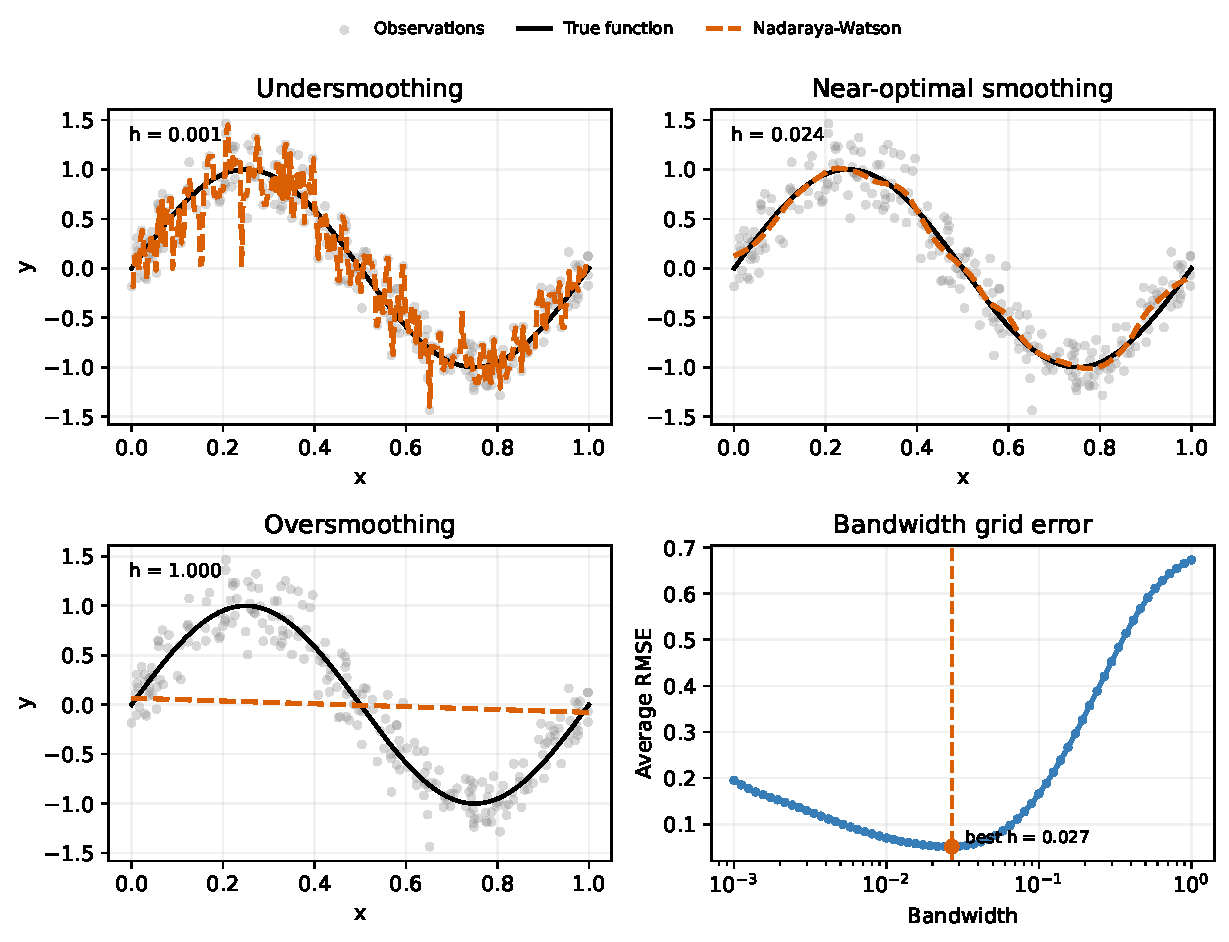
\includegraphics[width=\textwidth]{figures/fig_bandwidth_sensitivity.pdf}
\caption{Bandwidth sensitivity in Nadaraya-Watson smoothing with \(n=250\). The first three panels show the same data fitted with \(h=0.001\), \(0.024\), and \(1\). The last panel reports the average RMSE over a bandwidth grid and marks the empirical optimum.}
\label{fig:bandwidth}
\end{figure}

Figure~\ref{fig:bandwidth} displays the bias-variance trade-off in a single estimator. With \(h=0.001\), most fitted values are determined by only a few nearby observations, so the curve becomes highly variable. With \(h=0.024\), the local averaging is close to the empirical risk optimum for this design and noise level. With \(h=1\), the estimator averages over a very wide range and approaches a global mean-like trend, suppressing the sine-shaped signal. The grid-error panel shows the same phenomenon quantitatively: RMSE is high at very small bandwidths, decreases near the optimal region, and then increases as oversmoothing bias dominates.
\FloatBarrier

\subsection{Comparison across Methods}

The second experiment compares methods under three regression functions:
\[
m_1(x)=\sin(2\pi x),
\]
\[
m_2(x)=\sin(2\pi x)+2\exp\{-100(x-0.5)^2\},
\]
\[
m_3(x)=x(1-x)+1.5\exp\{-80(x-0.08)^2\}.
\]
The three cases represent a smooth periodic curve, a local spike, and a boundary feature.

\begin{figure}[H]
\centering
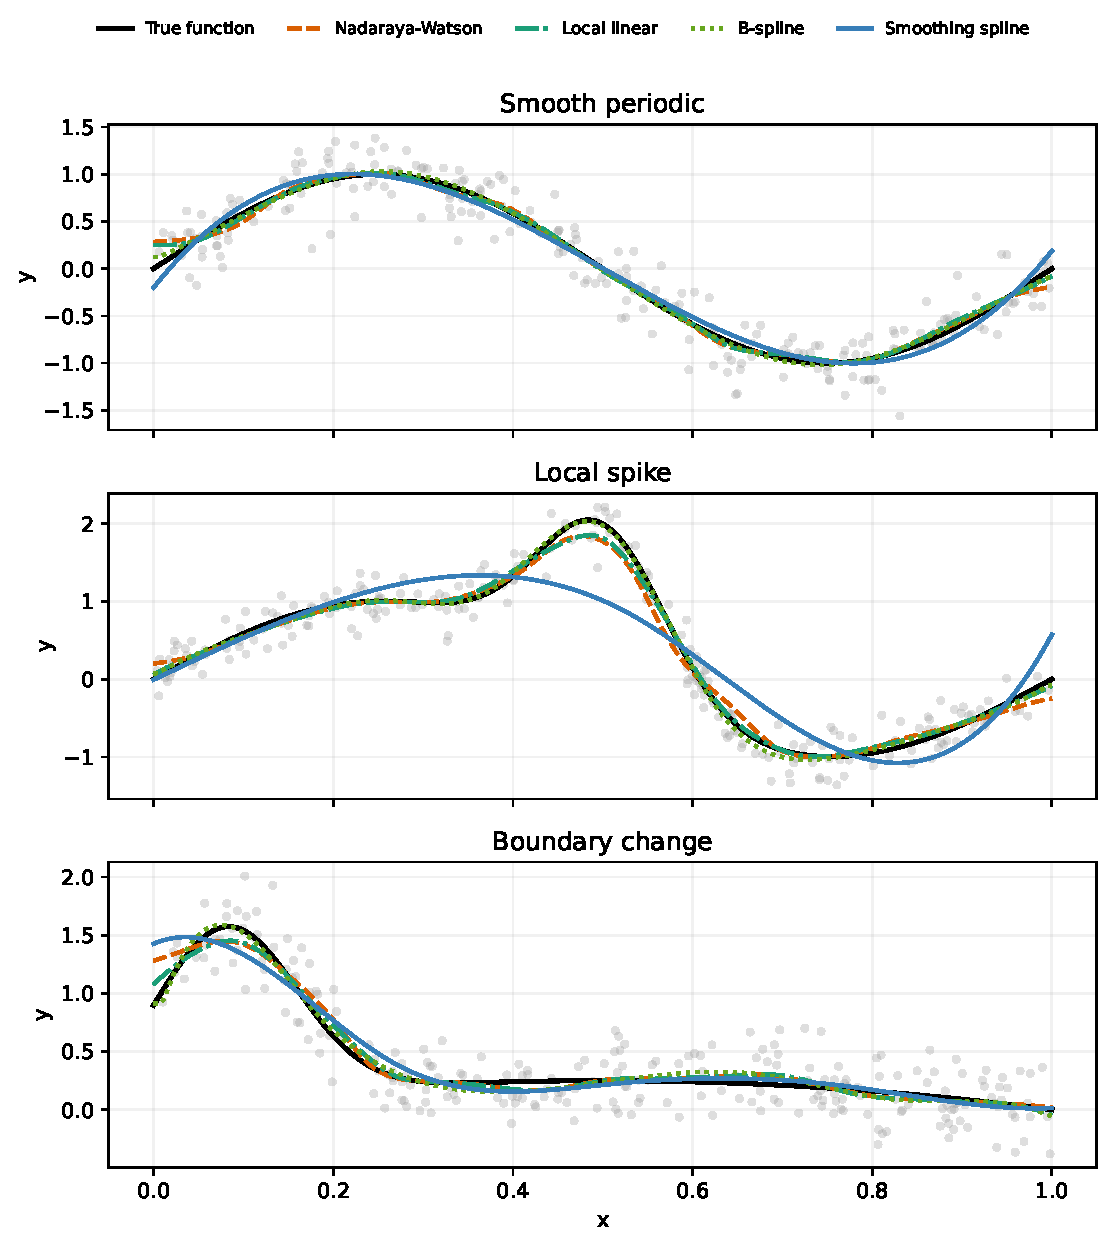
\includegraphics[width=0.86\textwidth]{figures/fig_method_fits.pdf}
\vspace{-0.6em}
\caption{Representative fitted curves for three regression functions.}
\label{fig:method-fits}
\end{figure}

\begin{figure}[H]
\centering
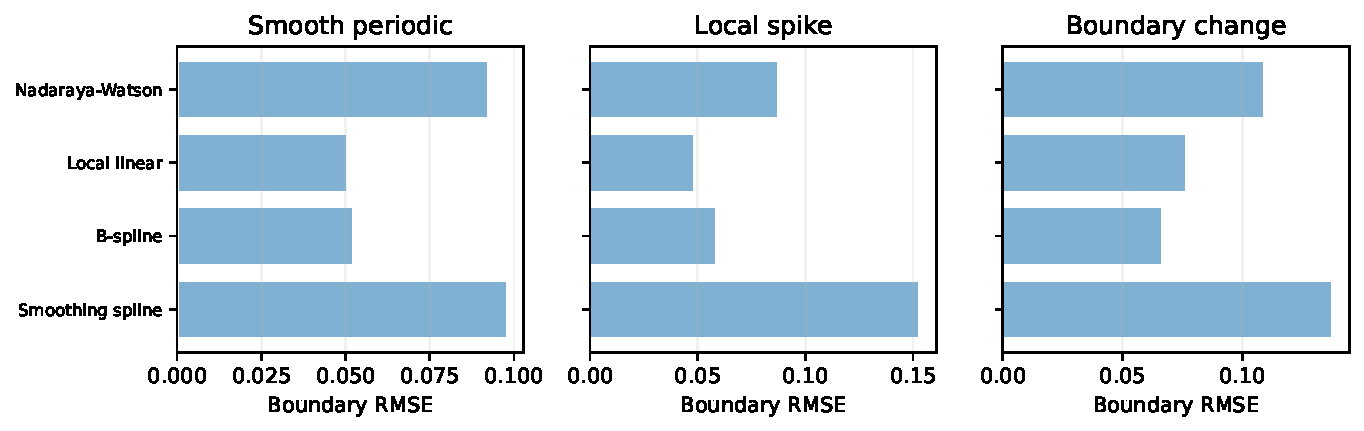
\includegraphics[width=0.88\textwidth]{figures/fig_boundary_rmse.pdf}
\caption{Boundary RMSE for representative smoothers in the method-comparison simulation. Boundary features expose the difference between local constant and local polynomial ideas.}
\label{fig:boundary-rmse}
\end{figure}

Figure~\ref{fig:method-fits} shows how the estimators differ beyond their average error. For the smooth periodic signal, the local linear and B-spline fits track the sinusoidal shape closely, while Nadaraya-Watson exhibits the characteristic boundary flattening of a local constant estimator. The smoothing spline is stable in the central region, but its global penalty can alter the fit near the endpoints when the selected smoothing level is relatively strong.

For the local spike, the distinction between local adaptation and global penalty becomes clearer. Nadaraya-Watson uses local averaging and therefore tends to attenuate the height of the spike when the bandwidth is not very small. Local linear regression follows the local change more effectively because the first-order term corrects local slope within the kernel window. The B-spline fit is comparatively stable because local basis support allows flexibility around the spike without forcing a high-degree global polynomial. In contrast, the smoothing spline can smooth through the spike when the roughness penalty treats the peak as excessive curvature rather than signal.

For the boundary-change function, Figure~\ref{fig:boundary-rmse} supports the boundary-bias discussion in Appendix~A3. Nadaraya-Watson has larger boundary RMSE because a one-sided kernel window near the edge leaves a local constant bias. Local linear regression reduces this error by estimating a local slope as well as an intercept. The B-spline fit also performs well in this setting because the basis can represent the boundary feature with moderate stability. Complete numerical summaries, including ISE, computation time, linear regression, polynomial regression, local quadratic regression, and compact RMSE tables, are reported in Appendix~B.
\FloatBarrier

\subsection{Influence of Noise Structure}

The third experiment continues to use \(Y_i=m(X_i)+\epsilon_i\), but fixes
\[
m(x)=\sin(2\pi x)+x
\]
and compares four noise structures:
\[
\epsilon_i\sim N(0,0.2^2),
\]
\[
\epsilon_i=0.2\,t_3/\sqrt{3},
\]
\[
\epsilon_i\sim N(0,\sigma^2(X_i)),\qquad \sigma(x)=0.1+0.4x,
\]
and
\[
\epsilon_i\sim0.95N(0,0.2^2)+0.05N(0,1.0^2).
\]
The goal is to examine how ordinary squared-loss smoothers behave under heavy tails, heteroscedasticity, and contamination.

\begin{figure}[H]
\centering
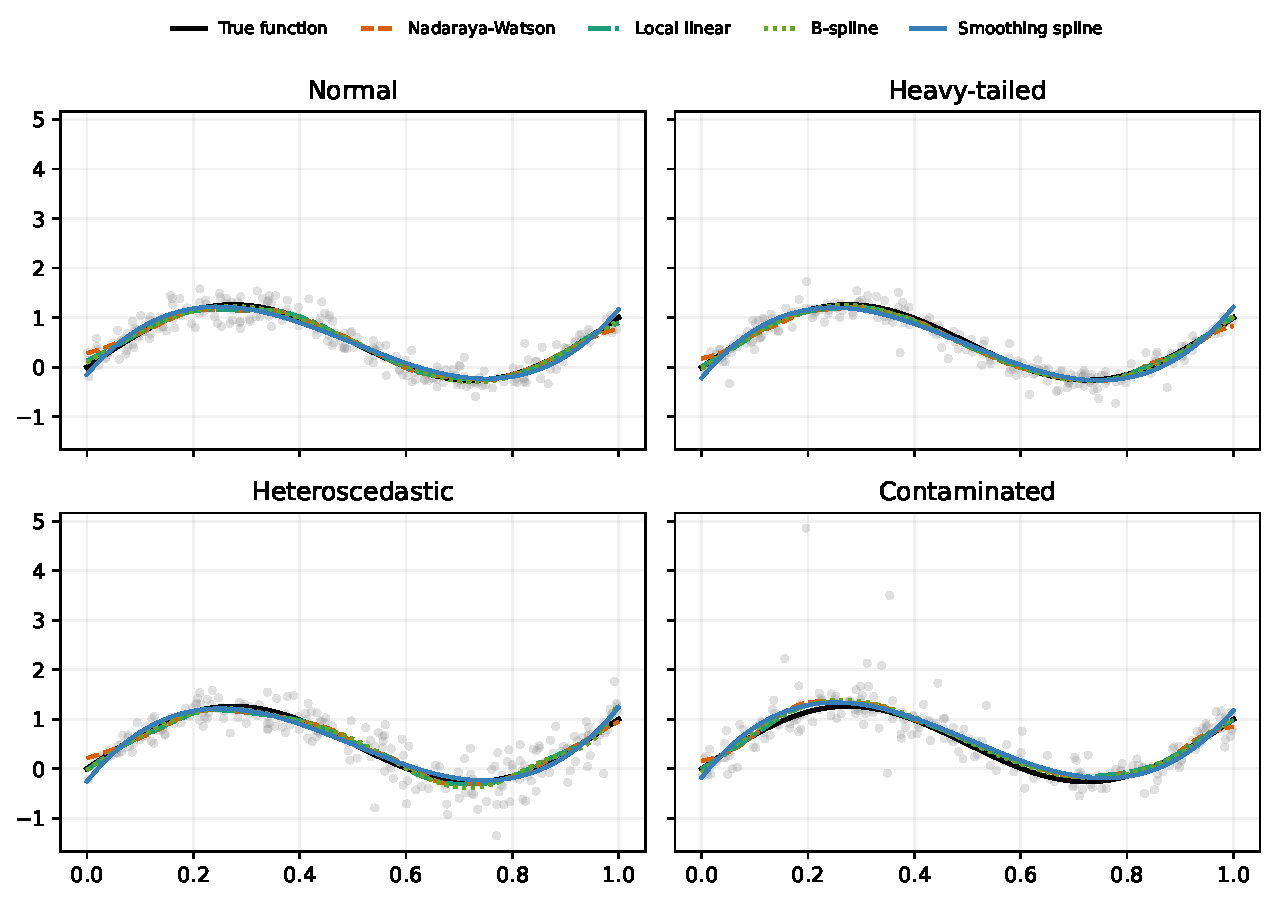
\includegraphics[width=0.94\textwidth]{figures/fig_noise_fits.pdf}
\caption{Representative fits under different noise structures.}
\label{fig:noise-fits}
\end{figure}

\begin{table}[H]
\centering
\caption{Average RMSE under different noise structures.}
\label{tab:noise-comparison}
\small
\begin{tabular}{lcccc}
\toprule
Noise & Nadaraya-Watson & Local linear & B-spline & Smoothing spline \\
\midrule
Contaminated & 0.0737 & 0.0629 & 0.0575 & 0.0796 \\
Heavy-tailed & 0.0588 & 0.0418 & 0.0366 & 0.0729 \\
Heteroscedastic & 0.0758 & 0.0663 & 0.0642 & 0.0841 \\
Normal & 0.0609 & 0.0444 & 0.0378 & 0.0731 \\
\bottomrule
\end{tabular}
\end{table}


\begin{figure}[H]
\centering
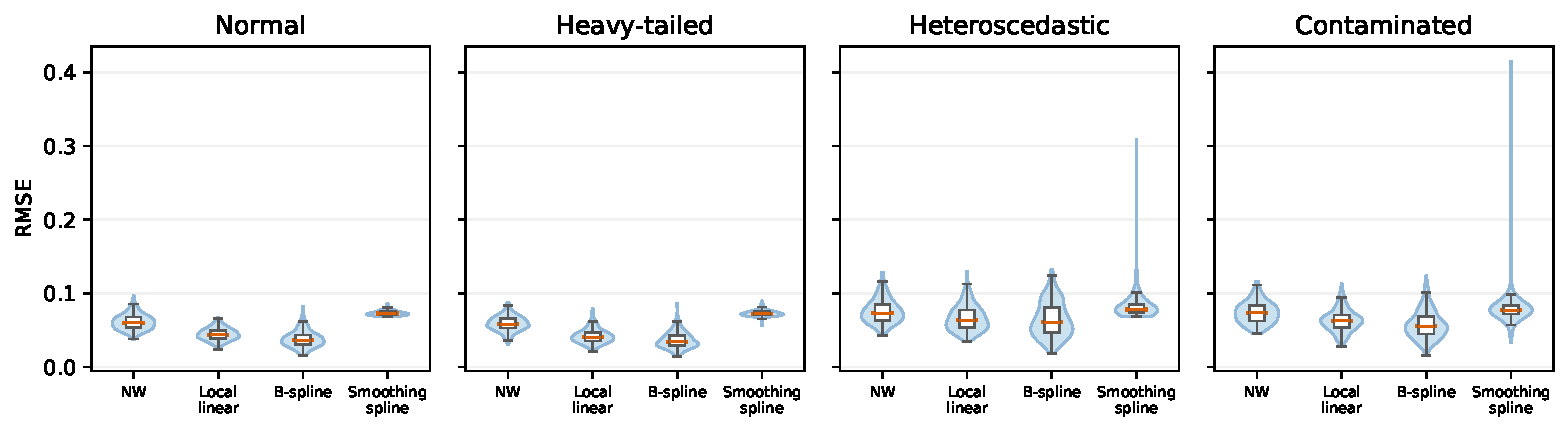
\includegraphics[width=0.96\textwidth]{figures/fig_noise_boxplots.pdf}
\caption{RMSE distributions under non-Gaussian noise. The violin and box summaries show how heavy tails, heteroscedasticity, and contamination change the sampling variability of mean-based smoothers.}
\label{fig:noise-boxplots}
\end{figure}

Under normal noise, the differences in Table~\ref{tab:noise-comparison} mainly reflect the smoothing mechanism rather than unusual observations. In this setting, B-splines and local linear regression have lower average RMSE than Nadaraya-Watson because they can represent local slope more effectively, while the smoothing spline is relatively conservative under the selected penalty.

Under heavy-tailed noise, all methods remain mean-based and are fitted under squared-loss criteria or local averages. Extreme errors can therefore affect the fitted curve even when they occur at only a few design points. Figure~\ref{fig:noise-fits} shows that the representative curves are still close to the truth, but Figure~\ref{fig:noise-boxplots} shows wider RMSE variability than in the normal case. The table again favors B-splines and local linear regression, suggesting that moderate local flexibility is useful when occasional large errors are present.

Under heteroscedastic noise, the variance increases with \(x\). A single bandwidth or a single smoothing penalty cannot be simultaneously optimal in low-variance and high-variance regions. This explains the larger RMSE values in Table~\ref{tab:noise-comparison} and the wider error distributions in Figure~\ref{fig:noise-boxplots}. 

The contaminated case is more abrupt: a small fraction of large errors visibly appears as isolated points in Figure~\ref{fig:noise-fits}, and the RMSE distributions become more variable. 

These results motivate robust extensions such as local LAD, local quantile smoothing, and robust spline fitting, discussed in Section~\ref{sec:discussion}. Detailed median absolute error results are reported in Appendix~B.
\FloatBarrier

\section{Real Data Analysis: Bike Sharing Dataset}
\label{sec:realdata}

The real-data analysis uses the Bike Sharing Dataset from the UCI Machine Learning Repository \citep{fanaee2014event}. The data record daily bike rental counts and weather or calendar variables. The response is \(cnt\), the total number of rentals. The main covariate is normalized temperature \(temp\). The analysis is exploratory: it studies the nonlinear association between temperature and rentals rather than fitting a full time-series or count-data model.

This distinction matters. The observations are time-ordered and may have seasonal dependence. The response is a count, so Poisson or negative-binomial additive models could be more natural for a full analysis. Here, squared-loss smoothing is used as a transparent way to compare the methods studied in the paper.

\begin{figure}[H]
\centering
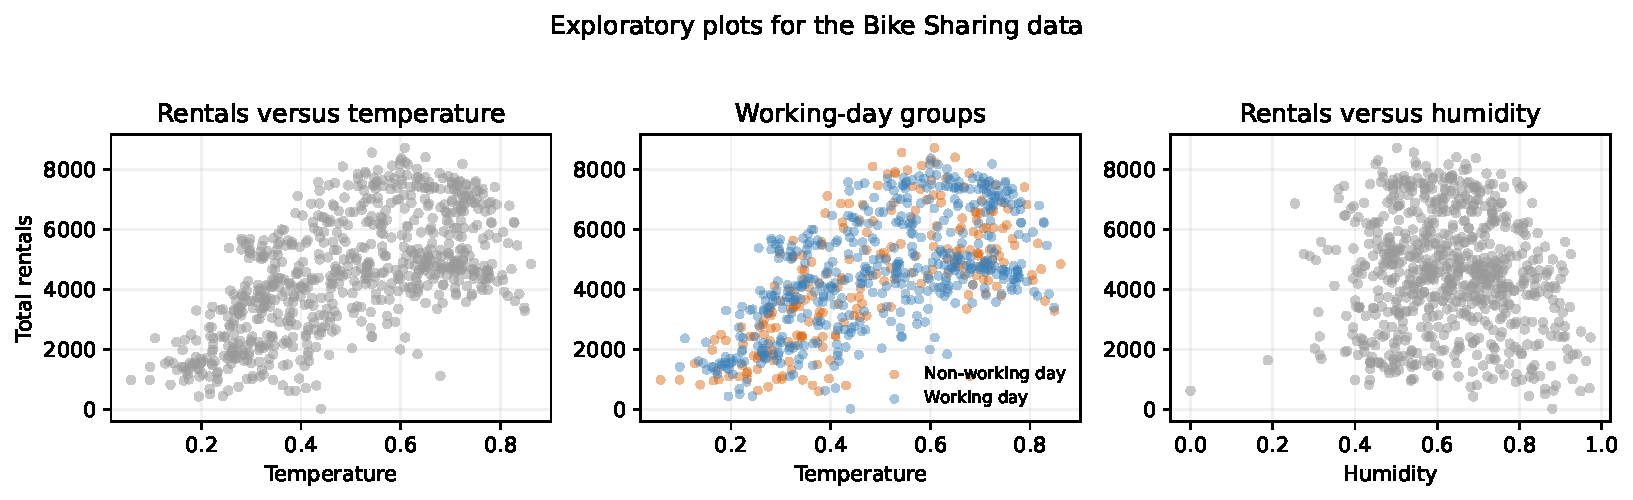
\includegraphics[width=\textwidth]{figures/fig_bike_exploratory.pdf}
\caption{Exploratory plots for the Bike Sharing data. Temperature has a visibly nonlinear association with total rentals.}
\label{fig:bike-exploratory}
\end{figure}

Figure~\ref{fig:bike-exploratory} suggests a nonlinear relationship between temperature and rentals. Rentals tend to increase as temperature rises, but the relationship is not well summarized by a single straight line. Humidity and working-day status also matter, but the main analysis remains one-dimensional to match the methods studied in the paper.

The fitted model is
\[
cnt_i=m(temp_i)+\epsilon_i.
\]
We compare linear regression, cubic polynomial regression, Nadaraya-Watson, local linear regression, B-spline regression, and smoothing spline. Kernel bandwidths, spline basis dimensions, and smoothing parameters are selected by five-fold cross-validation. The evaluation measures are cross-validated RMSE and MAE.

\begin{figure}[H]
\centering
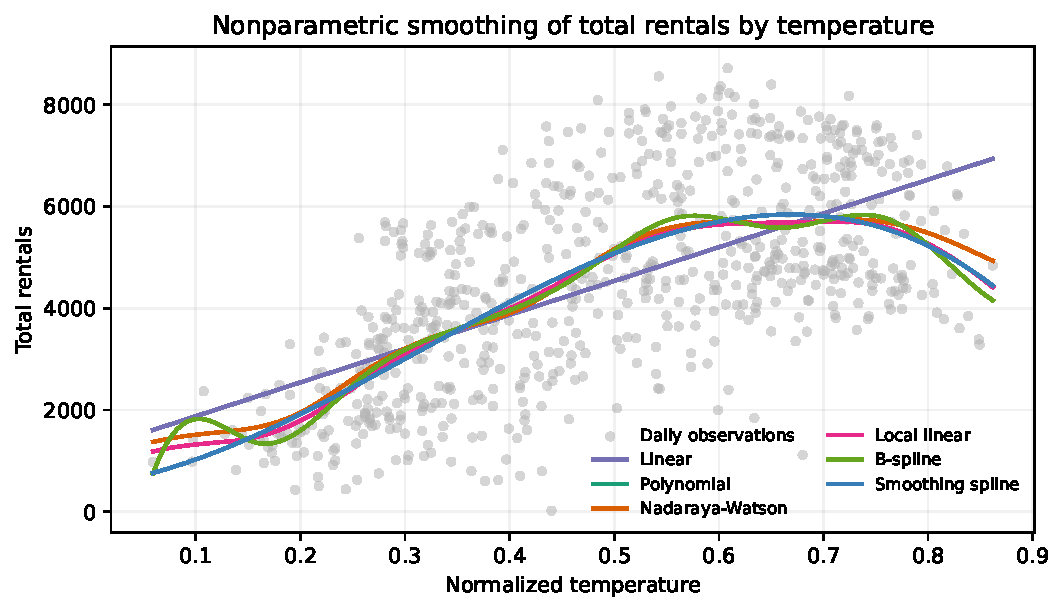
\includegraphics[width=0.86\textwidth]{figures/fig_bike_fits.pdf}
\caption{Fitted smoothing curves for total rentals as a function of temperature. Nonparametric smoothers reveal curvature that the linear model misses.}
\label{fig:bike-fits}
\end{figure}

\begin{table}[H]
\centering
\caption{Cross-validated errors for the Bike Sharing analysis.}
\label{tab:bike-cv}
\small
\begin{tabular}{lccc}
\toprule
Method & CV RMSE & CV MAE & Selected parameter \\
\midrule
Local linear & 1426.953 & 1188.686 & bandwidth=0.07 \\
B-spline & 1428.079 & 1186.589 & n\_knots=9 \\
Smoothing spline & 1428.594 & 1192.794 & smoothing\_factor=1 \\
Polynomial & 1428.594 & 1192.794 & degree=3 \\
Nadaraya-Watson & 1430.005 & 1194.859 & bandwidth=0.05 \\
Linear & 1512.434 & 1250.784 & None \\
\bottomrule
\end{tabular}
\end{table}


Figure~\ref{fig:bike-fits} and Table~\ref{tab:bike-cv} show that the nonparametric smoothers have similar cross-validated performance, while the linear model is weaker. The local linear and spline fits suggest increasing demand with temperature, with a tendency toward flattening at warmer values. The precise curve depends on the smoothing mechanism, which echoes the simulation results: real-data interpretation should consider both predictive error and curve stability.

\begin{figure}[H]
\centering
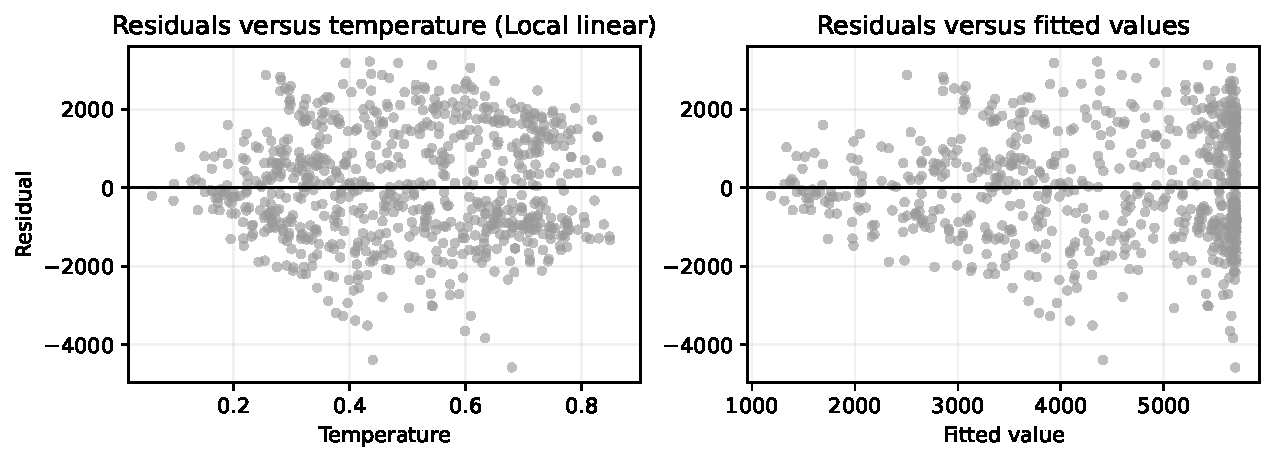
\includegraphics[width=0.95\textwidth]{figures/fig_bike_residuals.pdf}
\caption{Residual diagnostics for the best cross-validated smoother in the Bike Sharing analysis. Remaining structure reflects the limitations of a one-dimensional squared-loss model.}
\label{fig:bike-residuals}
\end{figure}

The residual plots in Figure~\ref{fig:bike-residuals} indicate that a one-dimensional smoother is only an exploratory description. Important variation remains, partly because demand depends on season, calendar variables, humidity, wind speed, and temporal dependence. A supplementary working-day comparison is included in Appendix~B.

The real-data analysis should therefore be interpreted as a shape analysis rather than as a final predictive model. Temperature is only one component of bike demand, and its marginal association with rentals may be affected by season, holidays, and weather variables. Moreover, the response is a count observed over time, so residual dependence and nonconstant variance are expected. These features do not invalidate the smoothing comparison, but they limit the causal or predictive conclusions that can be drawn from a one-dimensional squared-loss fit.

This example nevertheless illustrates the practical role of nonparametric smoothing. A linear model gives a simple increasing trend, while the nonparametric fits reveal curvature and flattening at warmer temperatures. The differences among local and spline fits are modest in cross-validated error but visible in curve shape. This mirrors the simulation results: in real applications, the smoothing parameter and the smoothing mechanism influence not only numerical accuracy but also the substantive interpretation of the fitted relationship.
\FloatBarrier
\FloatBarrier


\section{Discussion}
\label{sec:discussion}

\subsection{Smoothing Parameter Selection and Cross-validation}

The experiments show that smoothing parameter selection is both statistically central and practically delicate. Cross-validation is attractive because it is data-driven and targets predictive error. In the bandwidth experiment, the CV-like risk curve provides a useful empirical benchmark for distinguishing under- and over-smoothing. However, the prediction-optimal curve may not be the most interpretable curve. A curve selected only to minimize prediction error may contain local wiggles that are difficult to interpret substantively, while a slightly smoother curve may better summarize the dominant trend.

Finite-sample instability is another concern. When the sample is small, the design is uneven, or the noise is heavy-tailed or heteroscedastic, the selected bandwidth or penalty can vary noticeably across resamples. This does not make cross-validation invalid, but it means that a single selected value should not be treated as exact. In applied work, it is often more informative to report the selected value together with a small sensitivity analysis showing how the fitted curve changes nearby.

The practical implication is that smoothing parameter choice should combine prediction error, curve stability, and the scientific goal. If the goal is forecasting, CV risk may be the primary criterion. If the goal is interpretation, the analyst should also ask whether the selected curve preserves features at a meaningful scale and whether the conclusion is stable under nearby smoothing levels.

\subsection{Local Methods versus Global Spline Methods}

Local methods and global spline methods implement the same bias-variance principle through different mechanisms. Local kernel methods are direct and adaptive: they estimate the curve using observations near the target point. This makes them useful for local structure, but it also makes them sensitive to boundary truncation and sparse design regions. The boundary simulation illustrates this limitation for Nadaraya-Watson smoothing.

Spline methods impose structure through a basis or a roughness penalty over the whole domain. This often improves global stability and gives convenient measures of complexity, such as basis dimension or effective degrees of freedom. The cost is that global penalties may smooth away narrow peaks, as seen in the local-spike simulation for the smoothing spline. B-splines partly mediate this trade-off because their basis functions have local support, but knot number and placement still affect the fitted curve.

Therefore method choice should depend on the scientific question rather than only on RMSE. If boundary behavior or local slope is important, local linear regression may be preferable to local constant smoothing. If the goal is a stable global trend, spline methods may be more appropriate. If narrow local features are scientifically meaningful, the analyst should avoid overly strong global penalties and should examine fitted curves as well as error metrics.

\subsection{Robust Nonparametric Regression}

The methods compared in this paper are primarily mean-based and use squared-loss fitting or local weighted averages. This is appropriate under moderate noise with finite variance, but it can be fragile under heavy-tailed errors, heteroscedasticity, or contamination. The noise experiment shows that a smoother can have reasonable average RMSE under normal noise while becoming less stable when a small fraction of observations has much larger errors. This behavior is consistent with the robust-statistics perspective that squared loss gives large residuals disproportionate influence \citep{huber1964robust,huber2009robust}.

Robust nonparametric regression can respond to this limitation by changing either the local loss function or the target function. Local LAD regression replaces squared loss by absolute loss and targets a conditional median, making isolated large errors less influential. Quantile regression generalizes this idea by estimating conditional quantiles rather than the conditional mean \citep{koenker1978regression,koenker2005quantile}. Its local versions use kernel or local polynomial ideas to estimate \(Q_\tau(Y\mid X=x)\), which directly addresses heteroscedasticity because different quantile curves describe changes in conditional spread \citep{chaudhuri1991nonparametric,yu1998local}.

Robust smoothing can also retain a mean-regression target while controlling influence. Robust locally weighted regression combines local smoothing with resistant residual weighting \citep{cleveland1979robust}. Huber-type local regression keeps nearly quadratic behavior for small residuals but downweights large residuals, while robust spline procedures replace the squared residual term or modify the fitting criterion so that a small number of contaminated observations does not dominate the fitted curve. Recent reviews of robust nonparametric procedures emphasize the same point: when the noise is heavy-tailed or contaminated, robustness is part of the statistical model rather than a cosmetic post-processing step \citep{salibianbarrera2023robust}.

These extensions connect naturally to robust-statistics ideas such as ranks, quantiles, medians, and bounded-influence losses. They also clarify the role of Experiment~5.4. The heavy-tailed and contaminated cases do not merely increase numerical error; they question whether the conditional mean under squared loss is the most stable target for the data-generating mechanism. A full robust smoothing comparison is beyond the scope of this paper, but the simulations indicate why robust nonparametric regression is a natural next step rather than an unrelated extension.

\subsection{High-dimensional Extension and GAM}

The analysis deliberately focuses on one-dimensional smoothing. This keeps the bias-variance mechanism visible, but it also reveals a limitation. In higher dimensions, local neighborhoods become sparse rapidly, so kernel and local polynomial methods require much larger sample sizes to achieve the same resolution. This curse of dimensionality is a classical obstacle in nonparametric regression \citep{bellman1961adaptive,stone1982optimal,gyorfi2002distribution}. It explains why unrestricted multivariate smoothing is rarely a practical default for exploratory data analysis.

Generalized additive models offer a useful compromise \citep{hastie1990generalized,wood2017generalized}. By writing
\[
E(Y\mid X_1,\ldots,X_p)=\alpha+\sum_{j=1}^{p}f_j(X_j),
\]
they allow nonlinear marginal effects while avoiding a fully nonparametric multivariate surface. Each component can be estimated using spline smoothers, and the fitted functions remain interpretable. Modern GAM fitting uses smoothing-parameter selection and penalized likelihood ideas to extend this framework beyond Gaussian squared-loss regression \citep{wood2011fast,wood2016smoothing}. Recent software and model-interpretation work further reflects the practical value of additive structure for interpretable nonlinear modeling \citep{simpson2024gratia,arelbundock2024marginaleffects,kraus2024igann,mueller2024gamformer}.

The price is the additive assumption: interactions must be added explicitly if they are scientifically important. Even so, the Bike Sharing data is a natural setting for such an extension. Temperature, humidity, wind speed, seasonality, and working-day indicators are all plausible contributors to demand, and the response \(cnt\) is a count. A Poisson or negative-binomial additive model could therefore replace the one-dimensional squared-loss analysis by modeling several smooth effects jointly. This would preserve interpretability through component functions while respecting the count-response nature of the data more closely than ordinary least squares.

\section{Conclusion}
\label{sec:conclusion}

This paper reviewed nonparametric smoothing methods through a unified principle: smoothing parameters control the bias-variance trade-off. KDE makes the principle explicit through bandwidth, bias, variance, AMISE, and the optimal rate. Nadaraya-Watson and local polynomial regression extend local smoothing to regression. B-spline regression and smoothing splines express the same complexity control through basis dimension and roughness penalties.

The simulations confirm that smoothing choices have statistical consequences. Bandwidth changes the fitted curve and its risk, method structure affects local and boundary behavior, and noise structure can challenge ordinary mean-based smoothers. The Bike Sharing analysis illustrates both the value and the limitation of these methods: nonparametric smoothing reveals nonlinear temperature effects, but a one-dimensional squared-loss analysis cannot fully account for temporal dependence, count responses, and other covariates.

Several extensions would make the analysis more complete. First, nonparametric confidence bands or bootstrap-based uncertainty quantification would help distinguish stable curve features from sampling noise. Second, robust nonparametric regression would be valuable when heavy tails, heteroscedasticity, or contamination make squared-loss smoothing fragile. Third, adaptive bandwidths or spatially varying smoothing penalties could allow the estimator to use less smoothing in regions with sharp structure and more smoothing in regions where the signal is flat or the design is sparse. Finally, the Bike Sharing analysis could be extended to a GAM or an additive count model involving temperature, humidity, wind speed, and calendar variables. These directions all retain the main lesson of the paper: flexible smoothing should balance predictive performance, interpretability, and explicit complexity control.

\newpage
\bibliographystyle{apalike}
\bibliography{references}

\appendix
\section{Theoretical Derivations}

\subsection{KDE Bias, Variance, AMISE, and Bandwidth Rate}
\label{app:kde}

Assume \(f\) is twice continuously differentiable, \(K\) is symmetric, \(\int K(u)du=1\), \(\int uK(u)du=0\), \(\int u^2K(u)du=\mu_2(K)<\infty\), and \(R(K)=\int K^2(u)du<\infty\). Also assume \(h\to0\) and \(nh\to\infty\).

The expectation of the KDE is
\[
E\{\hat f_h(x)\}
=\int \frac{1}{h}K\left(\frac{x-t}{h}\right)f(t)dt.
\]
With \(u=(x-t)/h\), this becomes
\[
E\{\hat f_h(x)\}=\int K(u)f(x-hu)du.
\]
By Taylor expansion,
\[
f(x-hu)=f(x)-hu f'(x)+\frac{h^2u^2}{2}f''(x)+o(h^2).
\]
Using the moment conditions,
\[
E\{\hat f_h(x)\}=f(x)+\frac{h^2}{2}\mu_2(K)f''(x)+o(h^2).
\]
Thus
\[
\operatorname{Bias}\{\hat f_h(x)\}=O(h^2).
\]

For the variance,
\[
\operatorname{Var}\{\hat f_h(x)\}
=\frac{1}{n}\operatorname{Var}\{K_h(x-X)\}.
\]
The leading term is
\[
E[K_h^2(x-X)]
=\int \frac{1}{h^2}K^2\left(\frac{x-t}{h}\right)f(t)dt
=\frac{1}{h}\int K^2(u)f(x-hu)du
=\frac{f(x)R(K)}{h}+o(h^{-1}).
\]
Therefore
\[
\operatorname{Var}\{\hat f_h(x)\}
=\frac{f(x)R(K)}{nh}+o((nh)^{-1}),
\]
so the variance order is \(O((nh)^{-1})\).

Integrating the squared leading bias and the leading variance gives
\[
\operatorname{AMISE}(h)
=\frac{h^4}{4}\mu_2^2(K)R(f'')+\frac{R(K)}{nh},
\]
where \(R(f'')=\int \{f''(x)\}^2dx\). This has the form \(C_1h^4+C_2/(nh)\). Differentiating with respect to \(h\) gives
\[
4C_1h^3-\frac{C_2}{nh^2}=0,
\]
so
\[
h_{\mathrm{opt}}=\left(\frac{C_2}{4C_1}\right)^{1/5}n^{-1/5}\asymp n^{-1/5}.
\]

\subsection{Nadaraya-Watson as a Ratio of Kernel Estimates}

Let \(f_X(x)\) be the marginal density of \(X\). Define
\[
g(x)=m(x)f_X(x).
\]
Since \(m(x)=E(Y\mid X=x)\), the numerator can be estimated by
\[
\hat g(x)=\frac{1}{n}\sum_{i=1}^{n}K_h(X_i-x)Y_i,
\]
and the denominator by
\[
\hat f_X(x)=\frac{1}{n}\sum_{i=1}^{n}K_h(X_i-x).
\]
Taking the ratio gives
\[
\hat m_h(x)=\frac{\hat g(x)}{\hat f_X(x)}
=
\frac{\sum_{i=1}^{n}K_h(X_i-x)Y_i}
{\sum_{i=1}^{n}K_h(X_i-x)}.
\]
This is exactly the Nadaraya-Watson estimator.

\subsection{Why Local Linear Regression Helps at Boundaries}

Let \(u_i=X_i-x\) and \(w_i=K_h(X_i-x)\). The local constant estimator is the intercept in the weighted least squares problem
\[
\min_{\beta_0}\sum_{i=1}^{n}w_i(Y_i-\beta_0)^2,
\]
so
\[
\hat m_{0}(x)=\hat\beta_0=\frac{\sum_i w_iY_i}{\sum_i w_i}.
\]
Define the local sample moments
\[
S_k(x)=\sum_{i=1}^{n}w_i u_i^k,\qquad
T_k(x)=\sum_{i=1}^{n}w_i u_i^kY_i.
\]
Then \(\hat m_0(x)=T_0(x)/S_0(x)\).

Assume that \(m\) is twice continuously differentiable near \(x\), and write the local Taylor expansion
\[
m(X_i)=m(x)+m'(x)u_i+\frac{1}{2}m''(x)u_i^2+o(u_i^2).
\]
Conditioning on the design points and using \(E(Y_i\mid X_i)=m(X_i)\),
\[
E\{T_0(x)\mid X_1,\ldots,X_n\}
=m(x)S_0(x)+m'(x)S_1(x)+\frac{1}{2}m''(x)S_2(x)+o(S_2(x)).
\]
Therefore
\[
E\{\hat m_0(x)\mid X_1,\ldots,X_n\}-m(x)
=m'(x)\frac{S_1(x)}{S_0(x)}
\frac{1}{2}m''(x)\frac{S_2(x)}{S_0(x)}
o\!\left(\frac{S_2(x)}{S_0(x)}\right).
\]
At an interior point with a symmetric kernel window and a sufficiently regular design density, the leading contribution to \(S_1(x)\) cancels because positive and negative \(u_i\)'s receive symmetric weights. Thus the first-order term is negligible and the leading deterministic bias is of second order. At a boundary, however, the window is truncated: most observations lie on one side of \(x\). The cancellation in \(S_1(x)\) no longer holds, and \(S_1(x)/S_0(x)\) is typically of order \(h\). The local constant estimator can therefore retain a first-order boundary bias proportional to \(m'(x)h\).

Local linear regression instead solves
\[
\min_{\beta_0,\beta_1}
\sum_{i=1}^{n}K_h(X_i-x)
\{Y_i-\beta_0-\beta_1(X_i-x)\}^2.
\]
In the notation above, the normal equations are
\[
\begin{pmatrix}
S_0 & S_1\\
S_1 & S_2
\end{pmatrix}
\begin{pmatrix}
\hat\beta_0\\
\hat\beta_1
\end{pmatrix}
=
\begin{pmatrix}
T_0\\
T_1
\end{pmatrix},
\]
and hence
\[
\hat m_1(x)=\hat\beta_0
=\frac{S_2T_0-S_1T_1}{S_0S_2-S_1^2}.
\]
Using the same Taylor expansion,
\[
E\{T_0\mid X\}
=mS_0+m'S_1+\frac{1}{2}m''S_2+o(S_2),
\]
\[
E\{T_1\mid X\}
=mS_1+m'S_2+\frac{1}{2}m''S_3+o(S_3),
\]
where \(m\), \(m'\), and \(m''\) are evaluated at \(x\). Substitution gives
\[
E\{\hat m_1(x)\mid X\}
=m(x)
\frac{1}{2}m''(x)
\frac{S_2^2-S_1S_3}{S_0S_2-S_1^2}
o(h^2).
\]
The terms involving \(m'(x)\) cancel exactly:
\[
S_2(m'S_1)-S_1(m'S_2)=0.
\]
This cancellation is algebraic and does not require the local window to be symmetric. Consequently, local linear regression removes the first-order trend term that produces boundary bias in local constant smoothing. The remaining leading bias is governed by local curvature rather than by the local slope, which explains why local linear regression is usually preferred near boundaries.

\subsection{Smoothing Matrix and Effective Degrees of Freedom}

For a fixed smoothing parameter \(\lambda\), a smoothing spline solves
\[
\min_f
\sum_{i=1}^{n}\{Y_i-f(X_i)\}^2
+\lambda\int\{f''(t)\}^2dt.
\]
The representer theorem for this problem implies that the minimizer is a natural cubic spline with knots at the observed design points. Although the optimization is written over an infinite-dimensional function class, the solution can therefore be represented in a finite-dimensional spline basis:
\[
f(t)=\sum_{j=1}^{K}\theta_jB_j(t),
\]
where \(B_1,\ldots,B_K\) are natural cubic spline basis functions. Let \(B\) be the \(n\times K\) design matrix with entries \(B_{ij}=B_j(X_i)\), and let
\[
\Omega_{jk}=\int B_j''(t)B_k''(t)\,dt
\]
be the roughness penalty matrix. The smoothing spline criterion becomes
\[
\|\mathbf y-B\theta\|^2+\lambda\theta^\top\Omega\theta.
\]
Differentiating with respect to \(\theta\) yields
\[
-2B^\top(\mathbf y-B\theta)+2\lambda\Omega\theta=0,
\]
so the fitted coefficient vector is
\[
\hat\theta=(B^\top B+\lambda\Omega)^{-1}B^\top\mathbf y.
\]
The fitted values at the observed points are therefore
\[
\hat{\mathbf y}=S_\lambda\mathbf y.
\]
More explicitly,
\[
S_\lambda
=B(B^\top B+\lambda\Omega)^{-1}B^\top .
\]
The matrix \(S_\lambda\) is the smoothing matrix. Its trace,
\[
\operatorname{df}(\lambda)=\operatorname{tr}(S_\lambda),
\]
is called the effective degrees of freedom. It measures the sensitivity of the fitted vector to the observed response vector. If \(\lambda=0\) and the basis is sufficiently rich, the fit approaches an unpenalized spline regression and \(S_\lambda\) has a larger trace. As \(\lambda\) increases, directions in coefficient space with large roughness penalty are increasingly shrunk. In an orthogonalized basis this behavior has the schematic form
\[
\operatorname{df}(\lambda)
=\sum_j \frac{d_j}{d_j+\lambda\rho_j},
\]
where \(d_j\) represents information from the data and \(\rho_j\ge0\) represents the roughness penalty in the \(j\)-th direction. Each penalized term decreases as \(\lambda\) increases. Thus larger \(\lambda\) implies fewer effective degrees of freedom and a smoother fitted curve. This is the spline analogue of increasing the bandwidth in kernel smoothing: both reduce complexity, lower variance, and can increase bias.

\section{Supplementary Simulation Results}

\subsection{Full Tables for Simulation Experiments}

Tables~\ref{tab:method-comparison}, \ref{tab:method-comparison-full}, and~\ref{tab:noise-comparison-full} report the numerical summaries behind the simulation figures. They include the compact RMSE comparison moved from the main text, additional baseline methods, local quadratic regression, integrated squared error, computation time, and median absolute error where applicable.

\begin{table}[H]
\centering
\caption{Compact simulation comparison across regression functions.}
\label{tab:method-comparison}
\small
\begin{tabular}{lccc}
\toprule
Function & Method & RMSE & Boundary RMSE \\
\midrule
Boundary change & B-spline & 0.0514 & 0.0669 \\
Boundary change & Local linear & 0.0542 & 0.0767 \\
Boundary change & Nadaraya-Watson & 0.0659 & 0.109 \\
Boundary change & Smoothing spline & 0.0944 & 0.138 \\
Local spike & B-spline & 0.0483 & 0.0587 \\
Local spike & Local linear & 0.0795 & 0.0486 \\
Local spike & Nadaraya-Watson & 0.0919 & 0.0876 \\
Local spike & Smoothing spline & 0.384 & 0.153 \\
Smooth periodic & B-spline & 0.0385 & 0.0524 \\
Smooth periodic & Local linear & 0.0444 & 0.0507 \\
Smooth periodic & Nadaraya-Watson & 0.0576 & 0.0923 \\
Smooth periodic & Smoothing spline & 0.0731 & 0.098 \\
\bottomrule
\end{tabular}
\end{table}


\begin{table}[H]
\centering
\caption{Supplementary simulation comparison across regression functions.}
\label{tab:method-comparison-full}
\small
\begin{tabular}{lccccc}
\toprule
Function & Method & ISE & RMSE & Boundary RMSE & Time \\
\midrule
Boundary change & Local quadratic & 0.002353 & 0.04764 & 0.05848 & 0.003914 \\
Boundary change & B-spline & 0.002737 & 0.05144 & 0.06688 & 0.0008194 \\
Boundary change & Local linear & 0.003029 & 0.05417 & 0.07674 & 0.003651 \\
Boundary change & Nadaraya-Watson & 0.004412 & 0.06585 & 0.1091 & 0.0002153 \\
Boundary change & Smoothing spline & 0.009749 & 0.09444 & 0.1377 & 0.0001509 \\
Boundary change & Polynomial & 0.03128 & 0.1768 & 0.2924 & 0.0006707 \\
Boundary change & Linear & 0.07556 & 0.2749 & 0.3512 & 0.0003858 \\
Local spike & B-spline & 0.002462 & 0.04835 & 0.05871 & 0.0008308 \\
Local spike & Local quadratic & 0.002961 & 0.05345 & 0.05798 & 0.003943 \\
Local spike & Local linear & 0.006433 & 0.07954 & 0.04861 & 0.003673 \\
Local spike & Nadaraya-Watson & 0.008674 & 0.09191 & 0.08762 & 0.00022 \\
Local spike & Smoothing spline & 0.1475 & 0.3836 & 0.1532 & 0.0001036 \\
Local spike & Polynomial & 0.2454 & 0.4954 & 0.3105 & 0.0006694 \\
Local spike & Linear & 0.579 & 0.7609 & 0.7208 & 0.0003861 \\
Smooth periodic & Local quadratic & 0.001462 & 0.03708 & 0.04808 & 0.003957 \\
Smooth periodic & B-spline & 0.001608 & 0.03846 & 0.05244 & 0.000817 \\
Smooth periodic & Local linear & 0.002053 & 0.04438 & 0.05066 & 0.003692 \\
Smooth periodic & Nadaraya-Watson & 0.003406 & 0.05757 & 0.09232 & 0.0002203 \\
Smooth periodic & Smoothing spline & 0.005361 & 0.07312 & 0.09798 & 7.016e-05 \\
Smooth periodic & Polynomial & 0.005361 & 0.07312 & 0.09798 & 0.0006723 \\
Smooth periodic & Linear & 0.2024 & 0.4499 & 0.6233 & 0.0003829 \\
\bottomrule
\end{tabular}
\end{table}


\begin{table}[H]
\centering
\caption{Supplementary simulation comparison under different noise structures.}
\label{tab:noise-comparison-full}
\small
\begin{tabular}{lccc}
\toprule
Noise & Method & RMSE & Median absolute error \\
\midrule
Contaminated & B-spline & 0.05751 & 0.03645 \\
Contaminated & Local linear & 0.06294 & 0.04278 \\
Contaminated & Nadaraya-Watson & 0.07366 & 0.04382 \\
Contaminated & Smoothing spline & 0.07961 & 0.05629 \\
Heavy-tailed & B-spline & 0.03665 & 0.02455 \\
Heavy-tailed & Local linear & 0.04182 & 0.02865 \\
Heavy-tailed & Nadaraya-Watson & 0.05882 & 0.03251 \\
Heavy-tailed & Smoothing spline & 0.07294 & 0.05773 \\
Heteroscedastic & B-spline & 0.06425 & 0.03466 \\
Heteroscedastic & Local linear & 0.06632 & 0.04089 \\
Heteroscedastic & Nadaraya-Watson & 0.07578 & 0.04349 \\
Heteroscedastic & Smoothing spline & 0.08407 & 0.05748 \\
Normal & B-spline & 0.03783 & 0.02532 \\
Normal & Local linear & 0.04438 & 0.03098 \\
Normal & Nadaraya-Watson & 0.06087 & 0.03419 \\
Normal & Smoothing spline & 0.07309 & 0.05762 \\
\bottomrule
\end{tabular}
\end{table}


\subsection{Boundary Bias Experiment}

The supplementary boundary experiment uses
\[
m(x)=x,\qquad X_i\sim U(0,1),\qquad \epsilon_i\sim N(0,0.1^2).
\]
The sample size is \(n=250\) and the number of repetitions is \(R=200\). Nadaraya-Watson and local linear regression use the same bandwidth. The purpose is to isolate the boundary effect.

\begin{figure}[H]
\centering
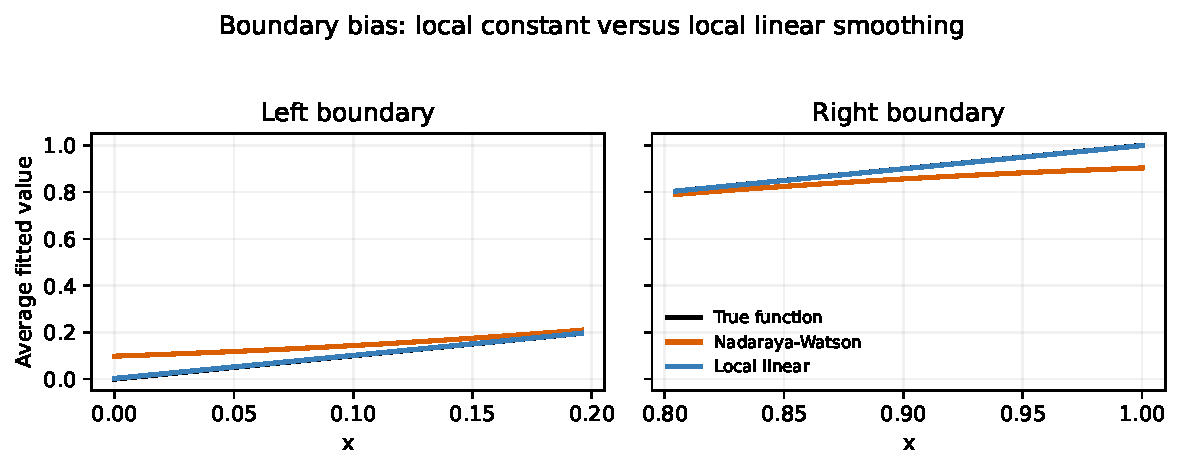
\includegraphics[width=0.86\textwidth]{figures/fig_boundary_bias.pdf}
\caption{Average fitted curves near the two boundaries in the supplementary boundary-bias experiment.}
\label{fig:boundary-bias}
\end{figure}

\begin{figure}[H]
\centering
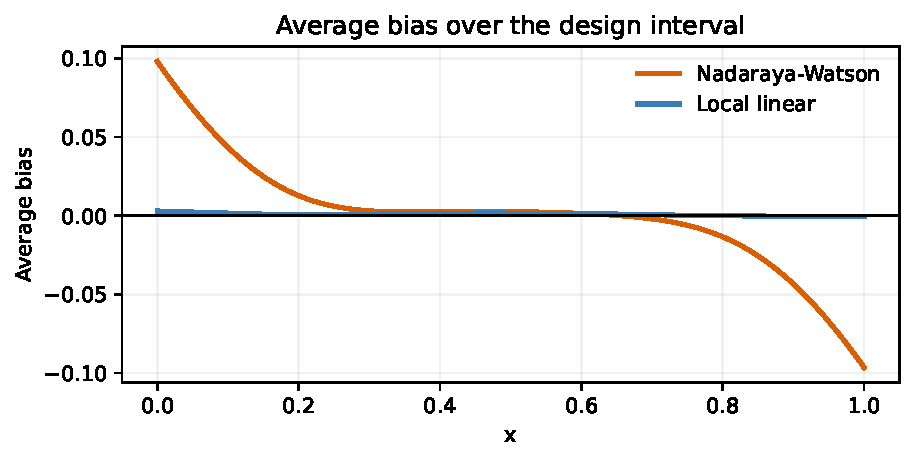
\includegraphics[width=0.72\textwidth]{figures/fig_boundary_bias_curve.pdf}
\caption{Average bias over the design interval in the supplementary boundary-bias experiment.}
\label{fig:boundary-bias-curve}
\end{figure}

\begin{table}[H]
\centering
\caption{Supplementary boundary-bias experiment.}
\label{tab:boundary-experiment}
\small
\begin{tabular}{lc}
\toprule
Method & Boundary RMSE \\
\midrule
Local linear & 0.0174 \\
Nadaraya-Watson & 0.0726 \\
\bottomrule
\end{tabular}
\end{table}


The results support the theoretical explanation in Appendix~A: local linear regression reduces the first-order boundary effect that appears in local constant smoothing.

\subsection{Working-day Supplement for the Bike Sharing Data}

\begin{figure}[H]
\centering
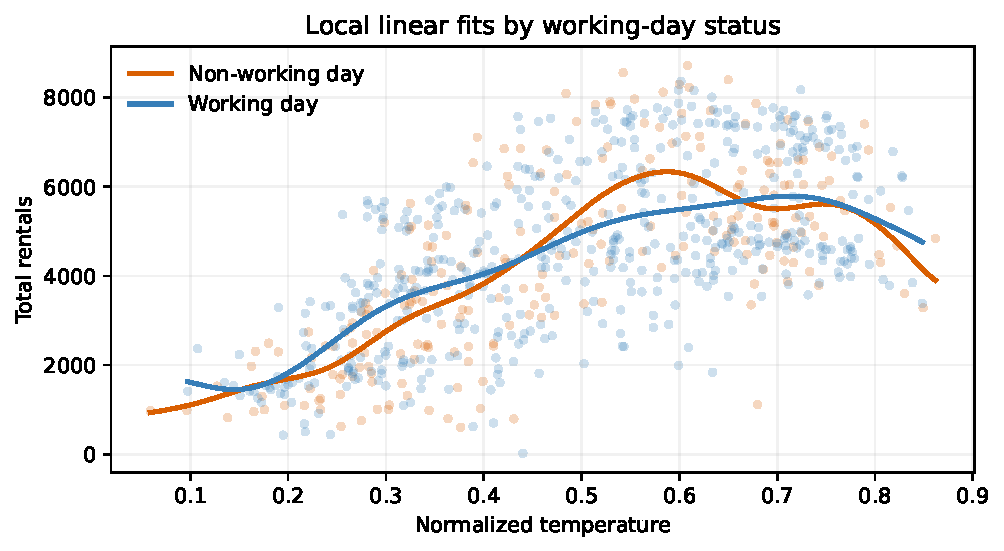
\includegraphics[width=0.72\textwidth]{figures/fig_bike_workingday.pdf}
\caption{Supplementary local linear fits by working-day status in the Bike Sharing data.}
\label{fig:bike-workingday}
\end{figure}

The grouped curves suggest that calendar structure affects rental counts. This supports the discussion that a full analysis of the Bike Sharing data should move beyond a one-dimensional smoother.

\section{Code Implementation}

The project repository is available at:
\url{https://github.com/YuxiaDing/NonparametricAnalysis-FinalProject}.

The code used in this paper is organized in the \path{code/} directory. The implementation is modular: \path{config.py} stores global settings such as random seeds, sample size, output paths, and tuning grids; \path{kernels.py}, \path{smoothers.py}, \path{metrics.py}, and \path{cv_utils.py} provide reusable functions for kernels, smoothing estimators, evaluation metrics, and cross-validation. The main simulation scripts are \path{simulate_bandwidth.py}, \path{simulate_methods.py}, \path{simulate_noise.py}, and \path{simulate_boundary.py}, corresponding respectively to the bandwidth-sensitivity experiment, the method-comparison experiment, the noise-structure experiment, and the supplementary boundary-bias experiment.

The real-data analysis is implemented in \path{real_data_bike.py}. This script loads the daily Bike Sharing data, produces exploratory plots, fits the smoothing methods used in the paper, computes cross-validated errors, and generates residual diagnostics. The scripts \path{make_all_figures.py} and \path{make_all_tables.py} serve as driver files for regenerating the figures and tables. Output figures are saved in \path{figures/}, and numerical summaries are saved in \path{tables/}.

The Bike Sharing Dataset is obtained from the UCI Machine Learning Repository and is associated with \citet{fanaee2014event}. The dataset can be downloaded from
\url{https://archive.ics.uci.edu/dataset/275/bike+sharing+dataset}.
This paper uses the daily data file \path{day.csv}. If the data are not included in the repository, the user should download the ZIP archive from UCI, extract it, and place \path{day.csv} under \path{data/Bike-Sharing-Dataset/}.

\end{document}
